\section*{Tests and metrics}

\subsection*{Classic Na\"ive Bayes vs Embeddings}

In figure \ref{fig:classic_nb_vs_embeddings} are represented the ROC curves obtained with the models 
using no preprocessing. The dataset split is here set to 80\% for the train set and 20\% for the test set.
The simplest approaches eventually brought the best results. In fact, using word embeddings, the final
accuracy was much lower than the one obtained with the classic Na\"ive Bayes with bag of words. 
Both the simple Bernoulli and the multinomial Na\"ive Bayes that counts words occurrences 
have reached the maximum accuracy with very similar results.

\begin{figure}[h!t]
    \centering
    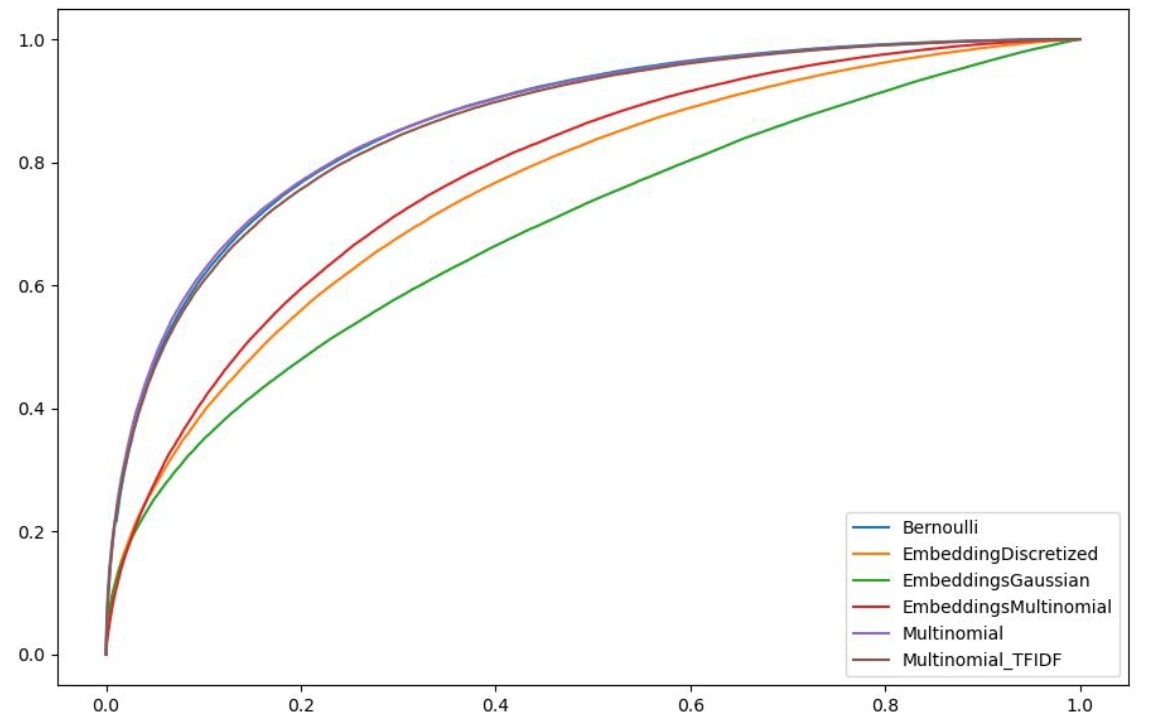
\includegraphics[scale=0.30]{../experiments/plots/classic_nb_vs_embeddings}
    \caption{ROC curves that compare the classic Na\"ive Bayes models with bag of words and
    word embedding approaches.}
    \label{fig:classic_nb_vs_embeddings}        
\end{figure}

In table \ref{tab:classic_nb_vs_embeddings} are shown some metrics about the models resulted from 
classic approaches. All of their performances are very similar with around 80\% of Accuracy and 
F1-score and 88\% of AUROC. 

\begin{table}[h!t]
    \centering
    \caption{Results obtained with bag of words Bernoulli and Multinomial models.}
    \label{tab:classic_nb_vs_embeddings}
    \begin{tabular}{c|ccc}
        \hline
        Model & Accuracy & F1 & AUROC \\
        \hline 
        Bernoulli & 0.797 & 0.799 & 0.880 \\ 
        Multinomial & 0.802 & 0.802 & 0.884 \\ 
        Multinomial TF-IDF & 0.805 & 0.804 & 0.886 \\ 
        \hline
    \end{tabular}
\end{table}

Additionally, some hyperparameter tuning has been applied. The intention has been to find the best n-grams
to maximize the final results.
In order to do that, 20\% of the dataset has been dedicated to the cross validation set.

\subsection*{Kaggle notebooks}

In this section we describe how we compared our models to a couple of top-rated notebooks on Kaggle.  We also tried to run these notebooks without removing stopwords from their datasets, to gain some further insight on the role their role in the learning process. 

The model we chose to compare to these notebooks is our most performing one: Multinomial Naive Bayes with Tf-Idf.  The first selected notebook on Kaggle is the most performing one to use the same technique ~/cite{notebook1}.  After resizing our dataset split to theirs, in order to make the comparison as equal as possible,  we were happy to see that it's area under the ROC score was slightly lower than ours,  as showed in table 2.  However, by running the same notebook without executing the preprocessing parts, its performance fairly improved.

\begin{table}[h!t]
    \centering
    \caption{Comparing our model to notebook ~/cite{notebook1},  with and without preprocessing}
    \label{tab:versus_metrics}
    \begin{tabular}{c|c}
        \hline
        Model & AUROC \\
        \hline 
        notebook & 0. 839 \\ 
        our model & 0.841 \\ 
        notebook without preprocessing & 0.849 \\ 
        \hline
    \end{tabular}
\end{table}

We also wanted to see if more complex models could capture the irregularities in word embeddings better than our Naive Bayes.  We searched Kaggle for the notebook with best results on word embeddings and found this one ~/cite{notebook2},  based on a LSTM neural network.  We were truly surprised to see that its accuracy was lower than the one reached by our Tf-Idf,  as showed in table 3. 

\begin{table}[h!t]
    \centering
    \caption{Comparing our model to notebook ~/cite{notebook2},  with and without stopword removal}
    \label{tab:versus_metrics}
    \begin{tabular}{c|c}
        \hline
        Model & Accuracy\\
        \hline 
        notebook & 0. 0.779 \\ 
        our model & 0.799 \\ 
        notebook without removing stopwords & 0.816 \\ 
        \hline
    \end{tabular}
\end{table}

However,  by emptying the lists of stopwords to be removed from the dataset and running the notebook again,  its accuracy enjoyed a significant boost.  The difference between the two executions of notebook [12] is a substantial result to support the intuition that some stopwords contain useful information that we want to keep in our dataset. 

\subsection*{Further tests}
We trained our model with a dataset and tested it against a different one, to this aim were used am IMDb dataset of cinematographic reviews ~\cite{data:imdb} and a Reddit one about various NFL games ~\cite{data:reddit}, results for the Bag-Of-Words Na\"ive Bayes (1,3)-gram model without preprocessing can be seen in figures \ref{fig:TwitterImdb} and \ref{fig:TwitterReddit}.

\begin{figure}[h!t]
    \centering
    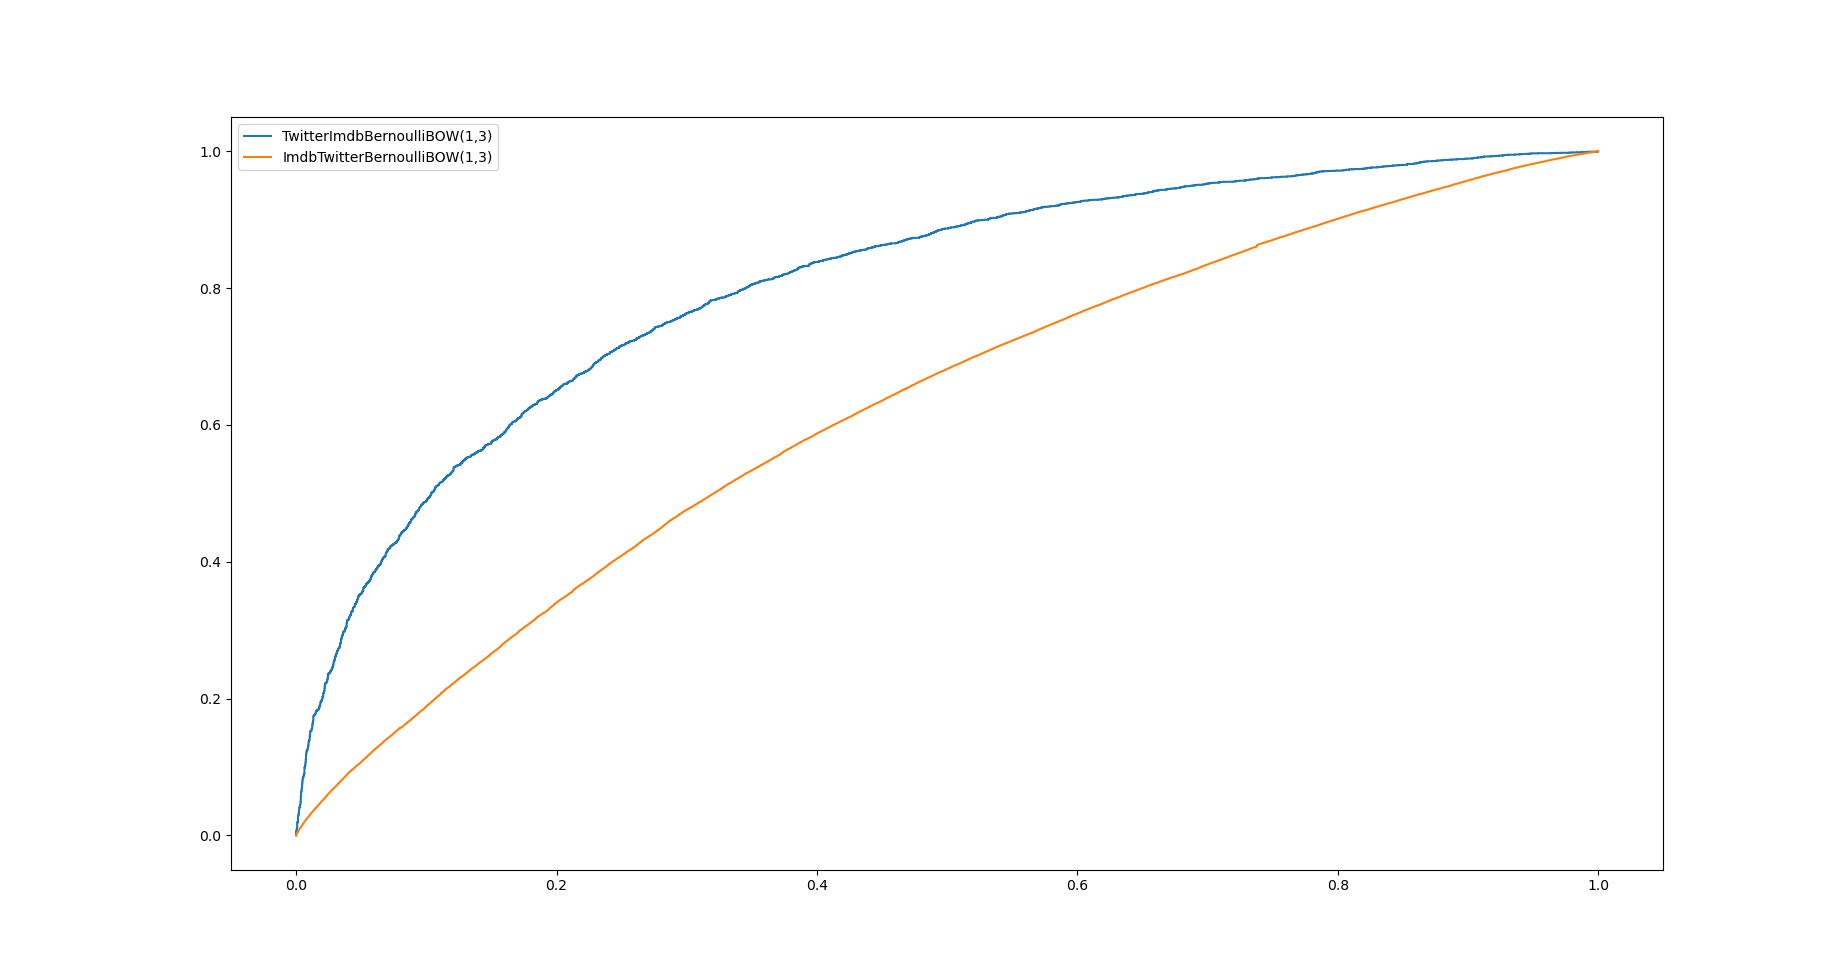
\includegraphics[scale=0.25]{../experiments/plots/ImdbTwitter}
    \caption{Comparison between Imdb-Twitter and Twitter-Imdb.}
    \label{fig:TwitterImdb}        
\end{figure}

\begin{figure}[h!t]
    \centering
    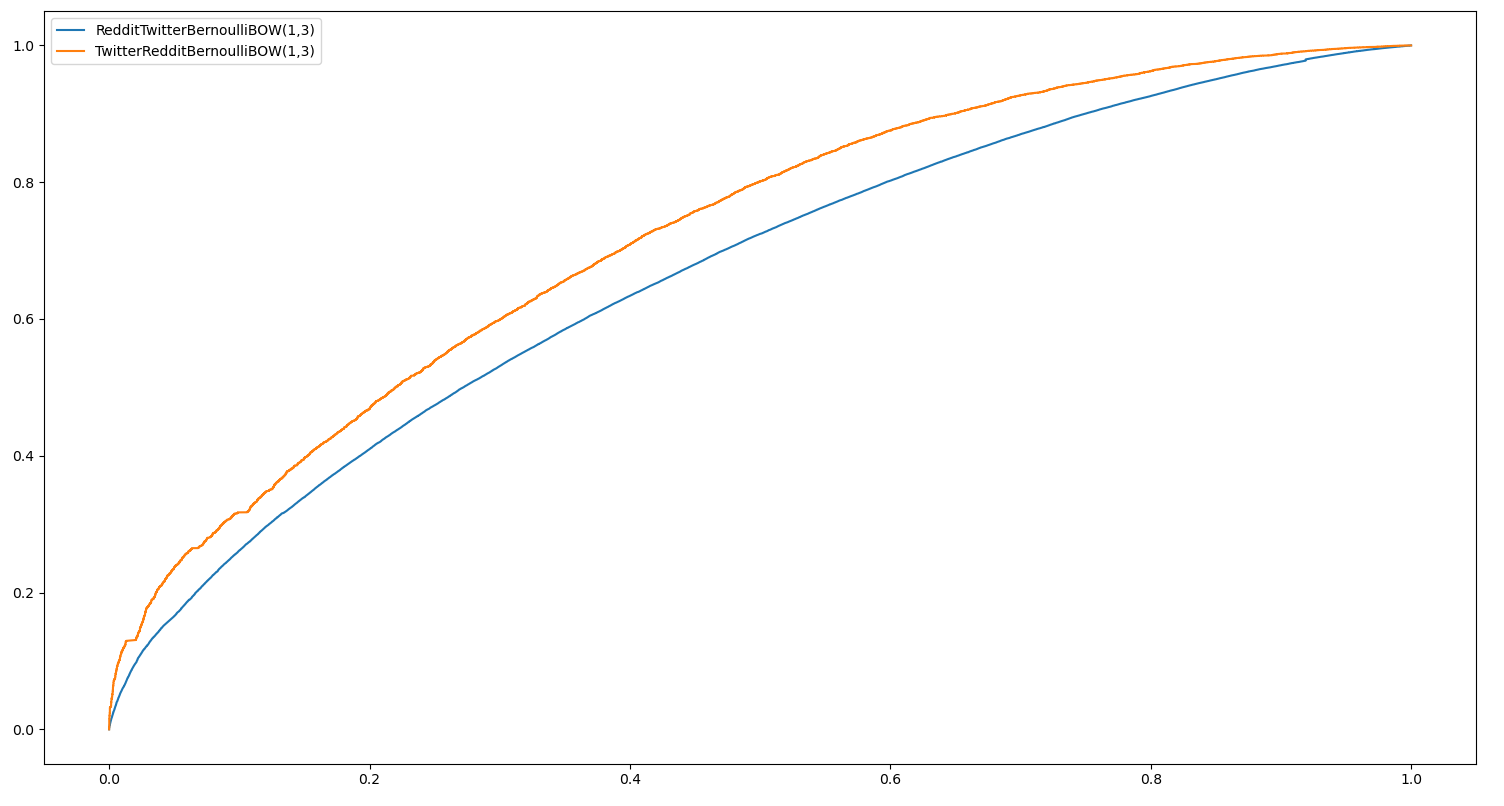
\includegraphics[scale=0.25]{../experiments/plots/RedditTwitter}
    \caption{Comparison betwen Reddit-Twitter and Twitter-Reddit.}
    \label{fig:TwitterReddit}
\end{figure}

This is something usually not done since different datasets will have different distributions hence we expect bad results and this is what we found except one single case.
Training our model with the Twitter dataset and testing it with the IMDb one strangely gives us rather good metrics, this can be seen in table \ref{tab:versus_metrics}, is exposed only the comparision betwen Twitter and IMDb since results are more interesting. 
This could happen since Twitter's dataset has a very large number of examples, other datasets other than being smaller are also very specific: the Reddit one is only about a specific set of american football games and the IMDb one is about cinematographic reviews, reasonably in this case lexicon is also more specific. 
Sentiment140 on the other hand covers a larger class of human language and is less prone to be biased.

\begin{table}[h!t]
    \centering
    \caption{Comparing metrics for some train test combinations.}
    \label{tab:versus_metrics}
    \begin{tabular}{c|ccc}
        \hline
        Train-Test & Accuracy & F1 & AUROC \\
        \hline 
        Twitter-IMDb & 0.732 & 0.723 & 0.806 \\ 
        IMDb-IMDb & 0.891 & 0.887 & 0.963 \\ 
        IMDb-Twitter & 0.550 & 0.330 & 0.625 \\ 
        Twitter-Twitter & 0.797 & 0.800 & 0.880 \\ 
        \hline
    \end{tabular}
\end{table}
